\documentclass[11pt]{book}

% Use the ETAMU physics style package
\usepackage{../../shared/styles/etamu-physics}

% Additional packages for Level 2
\usepackage{braket}  % For quantum mechanics notation

% Document metadata
\title{Level 2 Physics\\Instructor Manual}
\author{ETAMU Physics Department}
\date{\today}

\begin{document}

\frontmatter
\maketitle

\tableofcontents
\listoffigures

\chapter{Preface}

Welcome to the Level 2 Physics Instructor Manual. This manual covers advanced topics in electricity and magnetism, waves, optics, and modern physics, with comprehensive LaTeX examples for advanced physics typesetting.

\mainmatter

\chapter{Electromagnetic Theory}

\section{Maxwell's Equations}

\begin{tutorialbox}[title=Advanced Mathematical Notation]
For vector calculus and field theory, use:
\begin{verbatim}
\[ \nabla \cdot \vect{E} = \frac{\rho}{\epsilon_0} \]
\[ \nabla \times \vect{B} = \mu_0\vect{J} + \mu_0\epsilon_0\frac{\partial \vect{E}}{\partial t} \]
\end{verbatim}
\end{tutorialbox}

Maxwell's equations in vacuum:

\begin{align}
    \nabla \cdot \vect{E} &= \frac{\rho}{\epsilon_0} & \text{(Gauss's law)} \\
    \nabla \cdot \vect{B} &= 0 & \text{(No magnetic monopoles)} \\
    \nabla \times \vect{E} &= -\frac{\partial \vect{B}}{\partial t} & \text{(Faraday's law)} \\
    \nabla \times \vect{B} &= \mu_0\vect{J} + \mu_0\epsilon_0\frac{\partial \vect{E}}{\partial t} & \text{(Ampère-Maxwell law)}
\end{align}

\section{Electromagnetic Waves}

The wave equation for electromagnetic waves:
\[ \nabla^2 \vect{E} = \mu_0\epsilon_0 \frac{\partial^2 \vect{E}}{\partial t^2} \]

The speed of light: $c = \frac{1}{\sqrt{\mu_0\epsilon_0}} = \SI{3.00e8}{\meter\per\second}$

\begin{tutorialbox}[title=Scientific Notation with siunitx]
Use \texttt{siunitx} for scientific notation:
\begin{verbatim}
\SI{3.00e8}{\meter\per\second}
\SI{1.602e-19}{\coulomb}
\SI{6.626e-34}{\joule\second}
\end{verbatim}
\end{tutorialbox}

\chapter{Modern Physics}

\section{Quantum Mechanics}

\begin{tutorialbox}[title=Quantum Mechanics Notation]
Use the \texttt{braket} package for quantum notation:
\begin{verbatim}
\[ \braket{\psi|\phi} \]
\[ \bra{\psi} \hat{H} \ket{\psi} \]
\[ |\psi\rangle = c_1|0\rangle + c_2|1\rangle \]
\end{verbatim}
\end{tutorialbox}

The time-dependent Schrödinger equation:
\[ i\hbar \frac{\partial}{\partial t} \ket{\psi(t)} = \hat{H} \ket{\psi(t)} \]

For a particle in a box of length $L$:
\[ \psi_n(x) = \sqrt{\frac{2}{L}} \sin\left(\frac{n\pi x}{L}\right) \]
\[ E_n = \frac{n^2\pi^2\hbar^2}{2mL^2} \]

\section{Special Relativity}

The Lorentz factor:
\[ \gamma = \frac{1}{\sqrt{1 - v^2/c^2}} \]

Time dilation and length contraction:
\begin{align}
    \Delta t &= \gamma \Delta t_0 \\
    L &= \frac{L_0}{\gamma}
\end{align}

Energy-momentum relation:
\[ E^2 = (pc)^2 + (mc^2)^2 \]

\begin{tutorialbox}[title=Creating Spacetime Diagrams]
Use TikZ for spacetime diagrams:
\begin{verbatim}
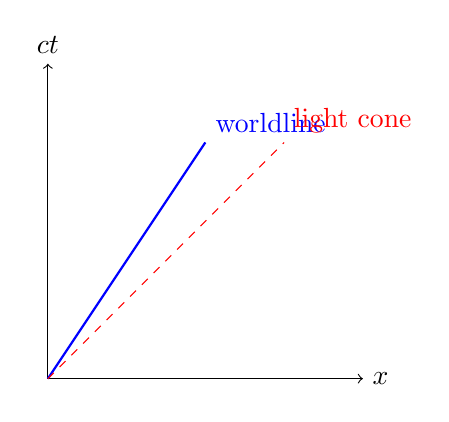
\begin{tikzpicture}
    \draw[->] (0,0) -- (4,0) node[right] {$x$};
    \draw[->] (0,0) -- (0,4) node[above] {$ct$};
    \draw[blue,thick] (0,0) -- (2,3) node[above right] {worldline};
    \draw[red,dashed] (0,0) -- (3,3) node[above right] {light cone};
\end{tikzpicture}
\end{verbatim}
\end{tutorialbox}

\chapter{Optics}

\section{Wave Optics}

For double-slit interference, the path difference is:
\[ \delta = d\sin\theta \]

Constructive interference occurs when:
\[ \delta = m\lambda, \quad m = 0, \pm 1, \pm 2, \ldots \]

\section{Geometric Optics}

The thin lens equation:
\[ \frac{1}{f} = \frac{1}{d_o} + \frac{1}{d_i} \]

Magnification:
\[ M = -\frac{d_i}{d_o} = \frac{h_i}{h_o} \]

\backmatter

\appendix

\chapter{Advanced LaTeX Techniques}

\section{Complex Equations}

For multi-line derivations, use the \texttt{align} environment:

\begin{verbatim}
\begin{align}
    F &= ma \\
      &= m\frac{dv}{dt} \\
      &= m\frac{d^2x}{dt^2}
\end{align}
\end{verbatim}

\section{Quantum Mechanics Symbols}

\begin{tabular}{ll}
    \toprule
    Symbol & LaTeX Command \\
    \midrule
    $\ket{\psi}$ & \texttt{\textbackslash ket\{\textbackslash psi\}} \\
    $\bra{\phi}$ & \texttt{\textbackslash bra\{\textbackslash phi\}} \\
    $\braket{\psi|\phi}$ & \texttt{\textbackslash braket\{\textbackslash psi|\textbackslash phi\}} \\
    $\hat{H}$ & \texttt{\textbackslash hat\{H\}} \\
    $\hbar$ & \texttt{\textbackslash hbar} \\
    \bottomrule
\end{tabular}

\end{document}